\documentclass[conference]{IEEEtran}
\IEEEoverridecommandlockouts
\usepackage{cite}
\usepackage{amsmath,amssymb,amsfonts}
\usepackage{algorithmic}
\usepackage{graphicx}
\usepackage{textcomp}
\usepackage{xcolor}
\begin{document}

\title{The Role of Gamification in UX Design}

\author{\IEEEauthorblockN{Jaewoong Suh}
\IEEEauthorblockA{\textit{AP Research} \\
\textit{Korea International School Jeju Campus}\\
Jeju, Republic of Korea \\
jwsuh25@kis.ac}
}

\maketitle

\begin{abstract}
Coming Soon
\end{abstract}

\begin{IEEEkeywords}
Gamification, UX Design, User Engagement, Progress Bars, Leaderboards
\end{IEEEkeywords}

\section{Literature Review}

\subsection{Introduction}

Enhancing HCI\footnote{HCI: Human-computer interaction, the study of how people interact with computers and other digital systems to improve usability, accessibility, and user experience.} has been a central focus since the inception of computing technology, as interface accessibility and user engagement continue to advance. Early HCI models, such as CLI\footnote{CLI: Command Line Interface, a text-based user interface where users interact with the computer through typed commands.} the required technical knowledge made it difficult for the majority of people to use the computer. A shift towards GUI\footnote{GUI: Graphical User Interface, allowing users to interact with devices through graphical elements rather than text commands.} \cite{curtis1989, fishkin2000} has revolutionized the way people communicate with technology, making interfaces more accessible through the use of icons, windows and direct manipulation elements. Simultaneously, the introduction of WYSIWYG\footnote{WYSIWYG: What You See Is What You Get systems are software design paradigms where the final output is displayed during the editing process} systems, such as Microsoft Word, reduced cognitive load, enabled real time feedback, and greatly improved usability \cite{marchionini1992}. With computing devices ubiquitized (e.g., smartphones, game consoles, embedded systems), the area of UI\footnote{UI: User Interface, the space where interactions between humans and machines occur, including elements like buttons, icons, and menus to facilitate user tasks.}
/UX\footnote{UX: User Experience, the overall experience and satisfaction a user has when interacting with a digital product or service.} has grown from providing functionality to crafting an engaging, immersive experience that not only holds and encourages user behavioral change \cite{deliu2017}.

This shift has increased interest in gamification\footnote{Gamification: The application of game-like elements, such as points, achievements, and rewards, in non-game contexts to increase user engagement and motivation.}, such as the use of game-like features like progress bars, achievements, and leaderboard, in non-game contexts to increase user engagement. Firstly known in the gaming industry, but now in education, e-commerce and tourism, gamification has become a way to improve the user experience in real life \cite{hiererra2022, clanton1998}. Thus, the principles of Cai, such as simplicity, naturalness, and user-friendly interfaces can be used to implement gamified elements that are consistent with natural user behavior and minimize cognitive load\footnote{Cognitive load: The amount of mental effort required to process information or complete a task.}, increase engagement and satisfaction level \cite{cai2009}.

Research in gamification within HCI emphasizes two key effects on users: structural and feedback ways of natural motivation and engagement \cite{healey2011, clanton1998}. Research has demonstrated that progress bars and badges can provide users with bite sized goals and instant feedback, achieving a sense of accomplishment that reinforces task completion and behavior repetition \cite{marchionini1992, chang2016}. We can see this in frameworks which frame entertainment and utilitarian effects of gamified systems, demonstrating that well-designed gamification can enhance user motivation without overloading or frustrating them \cite{deliu2017}.

While gamification’s potential to enhance UX has been increasingly validated, there are gaps regarding how it should be implemented, and how it affects engagement in web applications. Research in this area focuses at present on theoretical frameworks and basic gamified elements, but not on comprehensive evaluations in various applications and demographics \cite{kompaniets2020}. Therefore, this literature review, which studies HCI, behavioral psychology and UX to analyze studies across these domains to provide a clear understanding of how gamification should be used in order to create effective, user centered interfaces. In the context of UX (User Experience) design and HCI (Human-Computer Interaction), this study addresses the following question: How do game-inspired features like progress bars, achievements, and leaderboards on websites influence user behavior, specifically their likelihood of completing complex tasks such as sign-ups, checkouts, or content creation?

\subsection{Gamification in UX Design}

In UX design, gamification is adding game-inspired elements, such as progress bars, achievements, and leaderboards to the digital interfaces to encourage user engagement and motivation. They encourage users to be consistent through interaction and to be loyal to the service. \cite{clanton1998}.

Recent studies have highlighted two main ways gamification enhances UX: structural engagement and feedback mechanisms. Structural engagement is the organization of tasks into a series of steps that can be completed, with the aid of a progress bar providing immediate visual feedback that the task is being completed. These elements help users to continue to achieve incremental goals, which reinforce that users are doing something, and therefore users feel that they have accomplished something good and this will positively impact user retention \cite{marchionini1992, chang2016}. Badges and achievements are feedback mechanisms that validates user, rewarding users for completing tasks and incentivizing user interactions with the platform \cite{deliu2017, cai2009}. Such features facilitate user centered design by meeting cognitive needs\footnote{Cognitive needs: The mental requirements of users for information processing, understanding, and ease of use, which contribute to an efficient and satisfying interaction with digital systems.}
 and allowing for a smooth experience with low cognitive load.

Notably, Cai’s design principles of simplicity and naturalness, which focuses on the importance of minimizing interface interference, promote interaction by fitting design with natural user behavior \cite{cai2009}. This is the same intuitive game mechanics principle of Clanton in which obstacles and challenges can make an interface interesting without overwhelming the user. For instance, taking away controls initially and introducing it progressively simplifies the task. In addition, instant feedback helps attract the attention towards the task naturally, which leads to a good user experience \cite{clanton1998}.

In addition, including social elements such as leaderboards, which have demonstrated to increase engagement by giving users comparative performance data, provides users with a competitive angle. But researchers warn that leaderboards must be used carefully to avoid discouraging users who might feel too far behind to compete well. Risk mitigation can be done by personalizing leaderboards and segmenting them according to demographics of users \cite{saptaputra2021}.

In gamification in UX design, so long as the principles of simplicity and user centered feedback are balanced with, gamification has shown huge potential in raising user motivation and creating satisfying, engaging digital experiences. Nevertheless, the precise mechanisms by which gamified elements enhance user engagement in different applications and demographic groups are not entirely understood. In the following section, these challenges will be addressed and future directions for gamification in UX will be suggested.

\subsection{Challenges and Future Directions}

Gamification has great promise to increase user engagement, but it also presents specific challenges that need to be considered to make gamification work effectively. The one key challenge is to find that balance between the complexity of the gamified elements versus usability, in that overly complex designs will turn people away instead of engaging them. As it is Cai’s principles of simplicity and consistency that also point out that gamified interfaces should remain intuitive and accessible \cite{cai2009}.

Another challenge is the scalability\footnote{Scalability: The capability of a system, process, or application to handle increased demand or expansion without compromising performance or usability.} of gamified systems, and in particular, as data driven design approaches\footnote{Data-driven design: An approach that relies on user data and analytics to inform design decisions, enhancing personalization and effectiveness based on actual user behavior.} and adaptive user interfaces\footnote{Adaptive user interfaces: Interfaces that automatically adjust and customize elements in response to individual user behaviors, preferences, or real-time conditions to optimize user experience.} become more common. Real time data is used in an adaptive design to adjust user interface elements such as difficulty levels or provide customized feedback based on individual user progress. Studies on scalable cloud architectures\footnote{Cloud architectures: The design and structure of systems hosted on cloud platforms, enabling scalable, on-demand access to resources and services over the internet.} indicate, however, that this requires sophisticated backend systems capable of processing and responding to user data at scale \cite{oracle2023}. Such adaptive designs in gamification, however, necessitate that the backend infrastructure\footnote{Backend infrastructure: The server-side systems and databases that support application functionality, processing, and data management behind the scenes.}
 is implemented in such a way that a lag is not experienced and the user experience during peak usage times \cite{linuxfoundation} is smooth.

It also raises the risk of such things as over reliance on extrinsic rewards such as badges and leaderboards. If gamified elements are used too much, users can quickly get used to the external reward rather than the intrinsic one, and begin to lose motivation. The gamification strategies that should be effective should blend extrinsic motivators with the intrinsic ones, that is, providing users with a feeling of accomplishment, or providing meaningful interaction in the interface \cite{deliu2017, healey2011}.

Furthermore, little study has been done on psychological impacts of gamification on various users’ demographics. Despite the fact that past studies have demonstrated a positive impact on user motivation from elements such as progress bars and achievements, more comprehensive evaluation across age, cultural, and motivational demographics is called for. For instance, users younger users may be attracted to competitive or similar leaderboards, while older users may prefer collaborative or non-competitive aspects \cite{hiererra2022, kompaniets2020}. Specific user profiles can be tailored to gamified elements and inclusivity and disengagement prevented amongst a broader audience.

Future research on gamification in UX design could focus on personalized gamification, adaptive interfaces and cross-cultural studies of engagement. With increasing gamification of digital products, the question of how to best tailor these features for different audiences, and how to keep the users motivated over time, will become critical to developing user centered, effective and ethical UX designs.

\subsection{Conclusion}

This literature review focused on the role of gamification in UX design, and more importantly, the effects that game inspired elements (like progress bars, achievements, and leaderboards) can cause in regard to the user engagement and task completion. Previous work has suggested that gamification can inspire users to engage more, by providing the user with a sense of accomplishment via structured and feedback mechanisms. But all that is challenged, above all struggling to create balance between simplicity and complexity, and designing within a scalable system, no less than addressing the obsessive priority on extrinsic rewards.

This comes despite these advancements, however, gaps in the literature particularly relating to how demographic factors impact user response to gamified elements mean they are not readily applicable in wider environments. Thus, future work should focus on the development of adaptive and personalized interfaces, cross-cultural studies, and focus on inclusive design. As part of gamification today, these elements will continue to influence how we shape UX for many industry types, but their use will only be as good as the ethical and effective implementation of these elements for each of our diverse user groups.

\section{Research Methodology}

\subsection{Experimental Design}

To address the research question, a controlled A/B testing\footnote{A/B Testing: A experiment that randomly assigns participants to view one of two types of webpages or use one of two versions of an app} was used to compare their effectiveness. The experiment was performed on the currently existing web application, Joseon Space, using its own generic traffic, thus providing a more realistic approach to the experiment. Users of the site were randomly divided at the servers level to the several variants of the sign-up page with various aspects of the gamification included. This randomization also made it possible to reduce the influence of the users on the conditions they are exposed to.

\subsection{Participant Selection and Sample Size}
Population: All organic traffic to Joseon Space website with desktop and mobile devices. IP addresses of the users accessed Joseon Space was used to find their geographical locations\footnote{Geographic Location: The location of the user as determined through IP address, leveraging certain IP adress is allocated to certain regions.}. All this information was anonymized and analyzed according to ethical rules and regulations.

The necessary sample size was calculated using power analysis. Assuming a small-to-medium effect size (Cohen’s $d = 0.3$)\footnote{Cohen’s $d$: A number that shows how big the difference is between two groups, in a standardized way.}, and setting the error at 5\%\footnote{Significance Level: The chance of making a mistake by concluding there’s an effect when there isn’t (false positive).}, the analysis showed that at least 4,000 users were needed to have an 80\%\footnote{Statistical Power: The likelihood of detecting a real effect if it exists; chance of finding a true effect.}Statistical Power \cite{poweranalysis}.


\subsection{User Interface Conditions}

The study explored five experimental conditions:

\begin{itemize}
    \item \textbf{Control Group:} A standard sign-up page with no gamified elements.
    \item \textbf{Progress Bar Condition:} Included a visual progress bar\footnote{Progress Bar: A graphical representation of task completion progress, providing feedback on user advancement.} to indicate task completion.
    \item \textbf{Achievements Condition:} Displayed badges\footnote{Badges: Visual tokens awarded for achieving specific milestones, often used to motivate users.} upon completing sections of the form.
    \item \textbf{Combined Gamification Condition:} Integrated both gamified elements—progress.
\end{itemize}

All other design elements, including layout, navigation, and content, remained consistent across conditions.

\subsection{Metrics and Data Collection}

Data collection was performed using Ackee\footnote{Ackee: An open-source analytics tool for tracking user behavior without compromising privacy.}, integrated with Nuxt JS\footnote{Nuxt JS: A framework based on Vue.js for building server-rendered web applications.} and deployed via Docker\footnote{Docker: A platform for containerizing applications to ensure consistent deployment environments.}. PostHog\footnote{PostHog: A product analytics platform supporting A/B testing and user behavior tracking.} was used for managing A/B testing. The following key performance indicators (KPIs) were tracked:

\begin{itemize}
    \item \textbf{Completion Rate:} The proportion of users who successfully completed the sign-up process.
    \item \textbf{Form Completion Percentage:} The percentage of the form completed before abandonment by users who did not finish signing up.
    \item \textbf{Time Spent on Page:} The duration users remained on the sign-up page.
    \item \textbf{Bounce Rate:} The percentage of users who left the page without interacting.
\end{itemize}

User interactions were anonymized, and no personally identifiable information (PII)\footnote{PII: Personally Identifiable Information, data that can identify a specific individual.} was collected.

\subsection{Data Analysis Methods}

Several approaches were employed to make conclusions from the study on the basis of data analysis. Basic statistics were calculated to summarize key patterns, such as averages and differences, across the groups tested. A comparison of averages between two groups, like the time people spent on a page, was done using a method called a two-sample \( t \)-test\footnote{Two-Sample \( t \)-Test: A method to compare the average values of two groups and see if the difference is meaningful.}\cite{statology_ttest_anova}. To look at differences among more than two groups, the study used a technique called ANOVA \footnote{ANOVA: Analysis of Variance; a method for comparing differences across multiple groups to see if they are statistically significant.}\cite{statology_chisquare_anova}. This was followed by additional checks to find which specific groups had major differences.

For binary outcomes like whether user completed sign up, a chi-square test\footnote{Chi-Square Test: A method to analyze patterns in yes/no or other categorical data.} was used to understand the relation between presence of gamification elements and likelihood of completion \cite{builtin_ttest_chisquare}. Finally, regression analysis\footnote{Regression Analysis: A method that looks at how different factors, like location or device type, influence results.} assisted the study in controlling for other variables and understand the factors as influenced by gamification \cite{psu_regression}.

\subsection{Validity and Reliability}

To increase confidence of the results obtained following measures were made to design the study in a way that would provide accurate and dependable results. Randomization for A/B testing was employed in order to minimize researcher bias and potential. The study was conducted using a live website that had been up over 2 years to make the results relevant to practical settings rather than operational environments. Another source of reliability is that data was collected systematically and objectively with the use of automated analytics tools hence minimizing possible measurement errors. To ensure variation in usage was due to the device, and not the season or day of the week, the experiment was carried out over four weeks. Furthermore, bot traffic was filtered using IP-based detection algorithms\footnote{IP-Based Detection: Identifying non-human traffic based on IP address patterns.}, and all data were secured via encryption\footnote{Encryption: The process of encoding data to protect it from unauthorized access.}.

\subsection{Limitations}

Limitations of the study are as follows: First, based on the user base and design of the Joseon Space website, it is difficult to generalize and apply the results of the work in other related studies and on other platforms. Second, the use of IP-based geographic location, which can contain errors due to some users using VPN\footnote{VPN: Virtual Private Network, a service that masks a user's real IP address and encrypts their internet connection for privacy or security reasons.} or proxy\footnote{Proxy: An intermediary server that acts between a user and the internet, often used for anonymity, caching, or bypassing access restrictions.}. Third, while interaction from bots was extracted out, other legitimate interactions could have been excluded too due to users' IP ranges falling into IPs commonly associated with bot activity.

Such limitations can be mitigated by carrying out the A/B testing not only on the Joseon Space website (a Korean heritage tourism web application) but also on diverse web applications spanning various categories and user demographics. In addition, enhancing logic to more accurately detect bots using a holistic evaluation that incorporates not only IP but also user agent\footnote{User Agent: A string of information that a web browser or application sends to servers, indicating the type of browser, operating system, and sometimes device details.}, behavioral patterns, and other metadata\footnote{Metadata: Additional data providing information about other data, such as timestamps, browser details, and usage patterns, which can help identify anomalies or bots.}, can improve the bot detection algorithms.



\section{Results}
\label{sec:results}

The experiment analyzed data from 3,316 users per condition, measuring user engagement based on the number of fields completed.

\begin{figure}[h]
    \centering
    \begin{minipage}{0.49\linewidth}
        \centering
        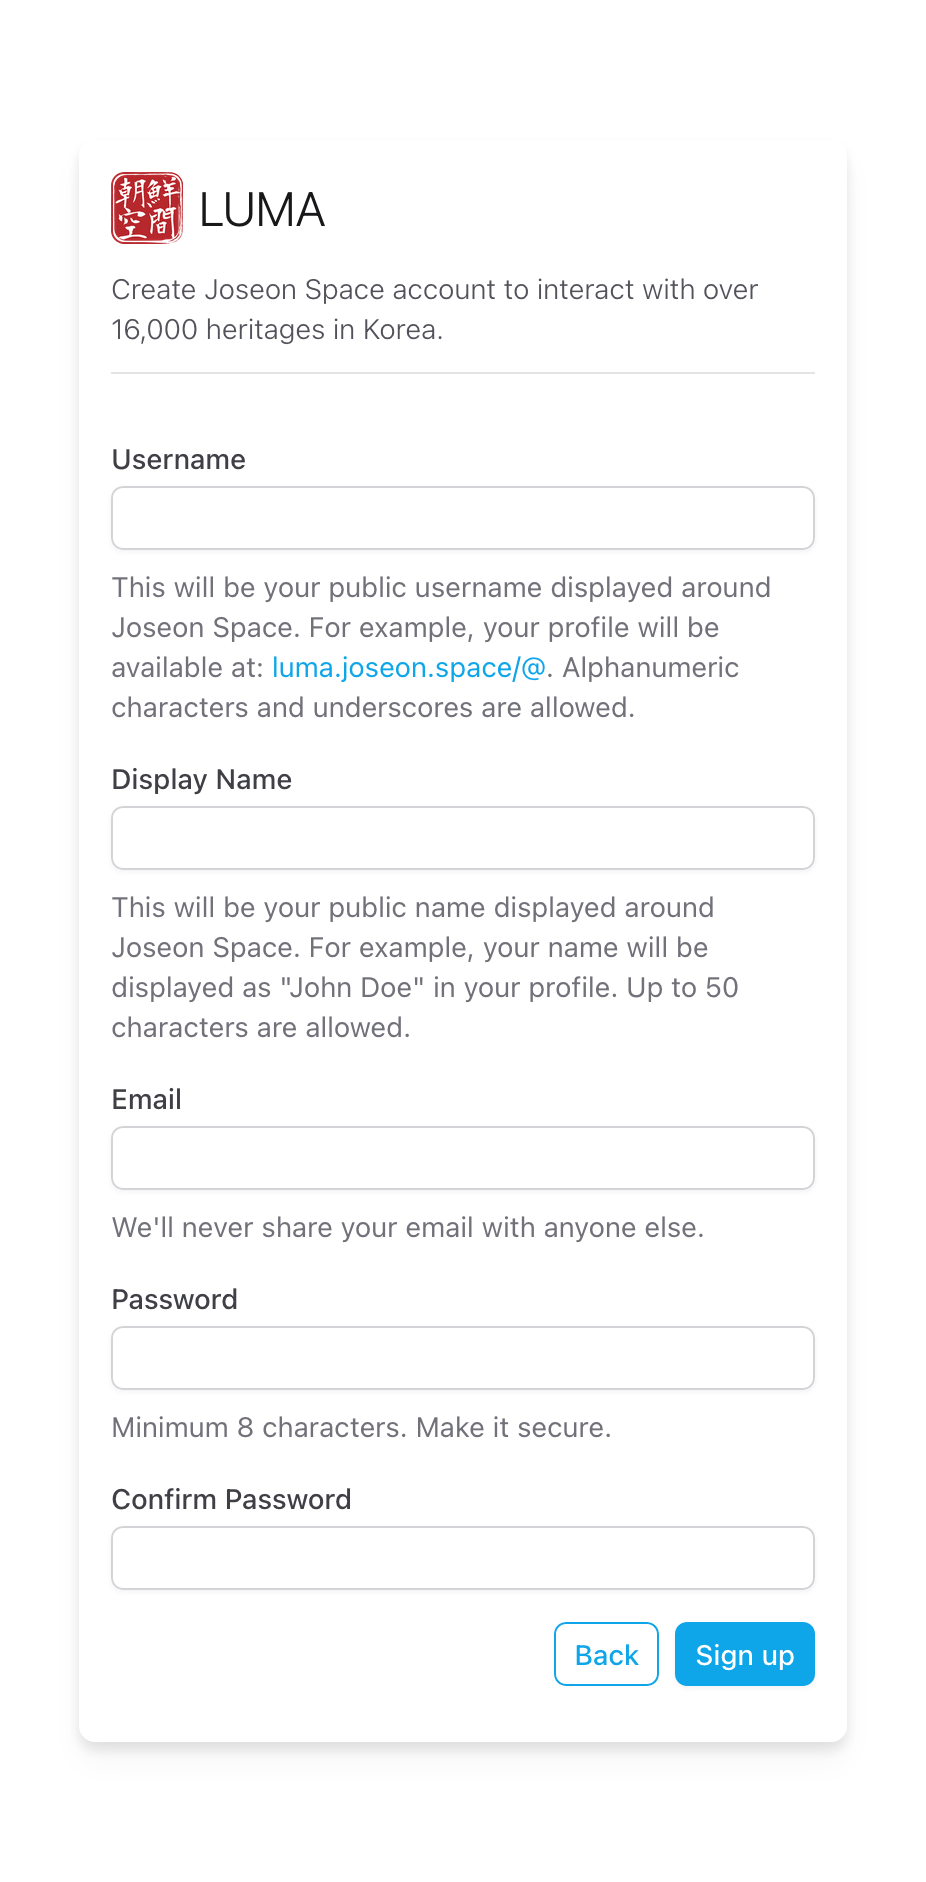
\includegraphics[width=\linewidth]{media/v1.png}
        \caption{Control: Normal sign-up}
    \end{minipage}
    \hfill
    \begin{minipage}{0.49\linewidth}
        \centering
        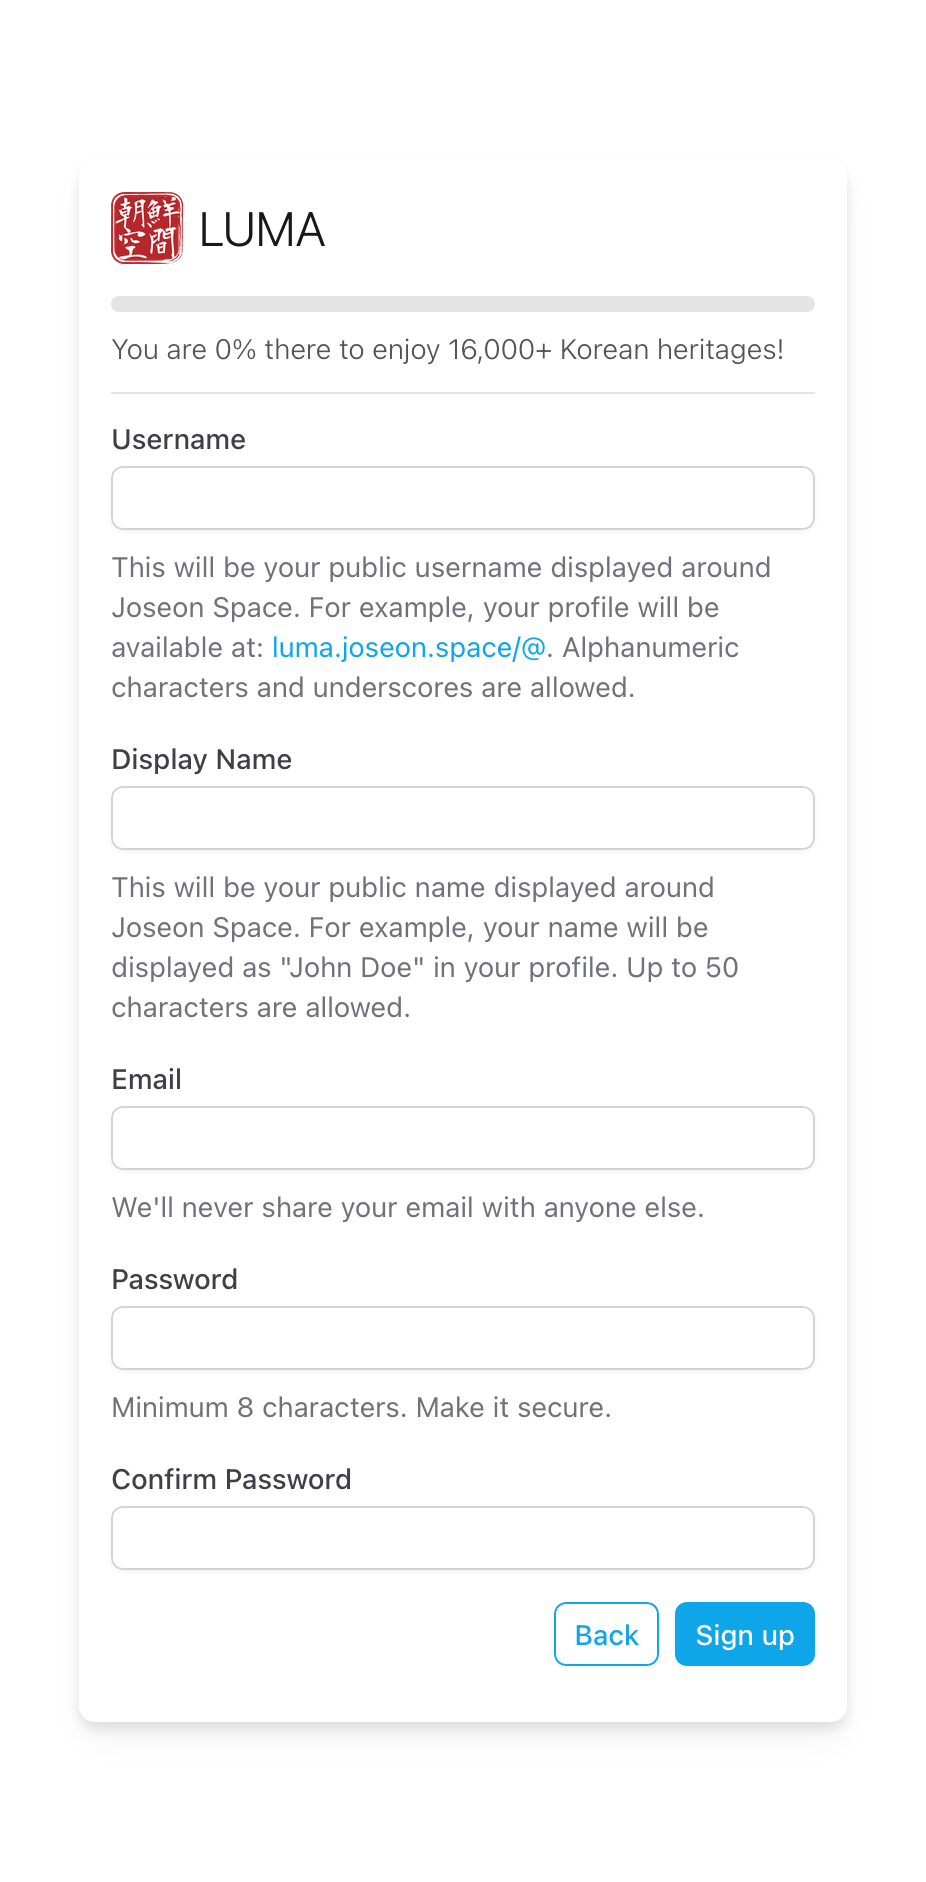
\includegraphics[width=\linewidth]{media/v2.png}
        \caption{Gamified sign-up}
    \end{minipage}
    \caption{Comparison of sign-up forms: control vs. gamified version}
\end{figure}


\subsection{Data Visualization}
\begin{figure}[!ht]
\centering
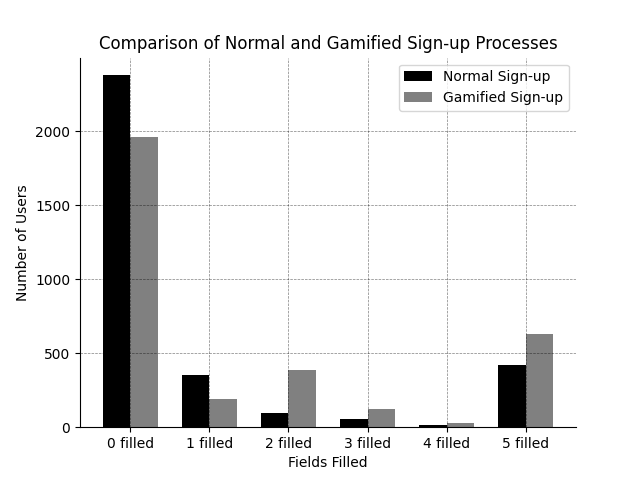
\includegraphics[width=3.5in]{media/sign_up_comparison.png}
\caption{Histogram comparing fields completed in normal and gamified sign-up processes.}
\label{fig:sign_up_comparison}
\end{figure}
The histogram in Figure~\ref{fig:sign_up_comparison} compares the distribution of fields completed between the normal (black bars) and gamified (gray bars) sign-up processes. The normal sign-up process shows a higher drop-off rate with fewer fields completed, while the gamified process demonstrates increased user engagement, with /Users/suhjae/Documents/KIS/AP Research/The Role of Gamification in UX Designa greater number of users completing more fields.

\subsection{Discussion of Findings}
The results suggest that incorporating game-inspired elements, such as progress bars positively influences user behavior. Users exposed to the gamified interface exhibited increased engagement, as evidenced by a higher number of completed fields and a lower abandonment rate.

These findings support the hypothesis that gamification enhances user motivation by providing visual feedback and incentives. However, further research is required to assess long-term user retention and whether gamified sign-ups improve conversion rates beyond initial interactions.

\section{Conclusion and Future Directions}

Through a controlled A/B testing, this study demonstrated that gamified elements---notably progress bars---significantly improve user engagement and completion rates. The data show that when feedback mechanisms reinforce incremental task completion, users experience higher motivation. These results confirm and extend previous research findings, suggesting that strategic use of gamified elements can offer an effective solution to common user dropout issues in digital interfaces.

\subsection{Potential Impact}
The observed behavioral changes indicate that incorporating clear goals, immediate feedback, and rewards can considerably influence user participation. In practical terms, this suggests that users, when presented with structured and visible progress, are more likely to persevere through onboarding tasks. This impact could reshape user expectations for online forms, sign-ups, and other digitally demanding interactions, leading to higher satisfaction levels across diverse demographics and contexts.

\subsection{Inferences}
These conclusions align with established human--computer interaction (HCI) principles and gamification frameworks outlined in the Literature Review \cite{cai2009, clanton1998, deliu2017}. The findings support the importance of simplicity, naturalness, and appropriately tailored feedback mechanisms by confirming the role of structural and feedback-based design elements.

\subsection{Limitation}
While this research confirms the short-term benefits of gamified features, several avenues remain open for further investigation:
\begin{itemize}
    \item \textbf{Other Gamification:} Data from the experiment only tested effect of progress bar in context of a sign up form. Experimenting with other gamification elements such as achievements and leaderboard on other context (beside signup) is needed
    \item \textbf{Cultural and Demographic Variations:} Cross-cultural research would refine understanding of how different age groups and cultural backgrounds respond to gamified features, ensuring broad applicability.
\end{itemize}


\begin{thebibliography}{00}

\bibitem{chang2016} J.-W. Chang and H.-Y. Wei, ``Exploring engaging gamification mechanics in massive online open courses,'' \textit{J. Educ. Technol. Soc.}, vol. 19, no. 2, pp. 177–203, 2016. [Online]. Available: http://www.jstor.org/stable/jeductechsoci.19.2.177

\bibitem{cai2009} X. Cai, ``Principles of human-computer interaction in game design,'' in \textit{Proc. 2009 Second Int. Symp. Comput. Intell. Des.}, 2009, vol. 2, pp. 92–95. [Online]. Available: https://doi.org/10.1109/ISCID.2009.171

\bibitem{clanton1998} C. Clanton, ``An interpreted demonstration of computer game design,'' \textit{DEMONSTRATIONS}, 1998. [Online]. Available: https://doi.org/10.1145/286498.286499

\bibitem{curtis1989} B. Curtis and W. Curtis, ``Engineering computer 'look and feel': User interface technology and human factors engineering,'' \textit{Jurimetrics}, vol. 30, no. 1, pp. 51–78, 1989. [Online]. Available: http://www.jstor.org/stable/29762155

\bibitem{deliu2017} D. Liu, R. Santhanam, and J. Webster, ``Toward meaningful engagement: A framework for design and research of gamified information systems,'' \textit{MIS Q.}, vol. 41, no. 4, pp. 1011–1034, 2017. [Online]. Available: https://www.jstor.org/stable/26630283

\bibitem{fishkin2000} K. P. Fishkin, A. Gujar, B. L. Harrison, T. P. Moran, and R. Want, ``Embodied user interfaces for really direct manipulation,'' \textit{Commun. ACM}, vol. 43, no. 9, pp. 74–80, 2000. [Online]. Available: https://doi.org/10.1145/348941.348998

\bibitem{healey2011} G. Healey, ``Persuasive design and building user engagement,'' \textit{Environ. Design Guide}, pp. 1–11, 2011. [Online]. Available: http://www.jstor.org/stable/26150788

\bibitem{hiererra2022} S. E. Hiererra, Meyliana, A. Ramadhan, and F. Purnomo, ``Prototype UX design: Mobile augmented reality application based on gamification for cultural heritage tourism,'' in \textit{Proc. 2022 8th Int. HCI and UX Conf. Indonesia (CHIuXiD)}, 2022, pp. 30–35. [Online]. Available: https://doi.org/10.1109/CHIuXiD57244.2022.10009802

\bibitem{kompaniets2020} V. Kompaniets, A. Lyz, and A. Kazanskaya, ``An empirical study of goal setting in UX/UI-design,'' in \textit{Proc. 2020 IEEE 14th Int. Conf. Appl. Inf. Commun. Technol. (AICT)}, 2020, pp. 1–5. [Online]. Available: https://doi.org/10.1109/AICT50176.2020.9368570

\bibitem{linuxfoundation} The Linux Foundation, ``Services, load balancing, and networking,'' \textit{Kubernetes}, n.d. [Online]. Available: https://kubernetes.io/docs/concepts/services-networking/

\bibitem{marchionini1992} G. Marchionini, ``Psychological dimensions of user-computer interfaces,'' \textit{Educ. Technol.}, vol. 32, no. 1, pp. 55–56, 1992. [Online]. Available: http://www.jstor.org/stable/44427588

\bibitem{oracle2023} Oracle, ``Design for scalability,'' \textit{Oracle Help Center}, Aug. 30, 2023. [Online]. Available: https://docs.oracle.com/en/solutions/oci-best-practices/design-scalability1.html

\bibitem{poweranalysis} Meera, ``Power Analysis, Statistical Significance, \& Effect Size,'' MEERA, n.d. [Online]. Available: https://meera.seas.umich.edu/power-analysis-statistical-significance-effect-size.html

\bibitem{ramey2000} J. Ramey, ``Guidelines for web data collection: Understanding and interacting with your users,'' \textit{Tech. Commun.}, vol. 47, no. 3, pp. 397–410, 2000. [Online]. Available: http://www.jstor.org/stable/43748887

\bibitem{saptaputra2021} E. H. Saptaputra, A. W. Utoyo, and N. Karlna, ``Gamification analysis in UI and UX for parking spot apps,'' \textit{J. Games, Game Art, Gamification}, 2021.

\bibitem{statology_ttest_anova} Statology, ``What is the difference between a t-test and an ANOVA?'', [Online]. Available: https://www.statology.org/what-is-the-difference-between-a-t-test-and-an-anova/. Accessed: Dec. 8, 2024.

\bibitem{statology_chisquare_anova} Statology, ``Chi-Square vs. ANOVA: Differences,'' [Online]. Available: https://www.statology.org/chi-square-vs-anova/. Accessed: Dec. 8, 2024.

\bibitem{builtin_ttest_chisquare} Built In, ``T-Test vs. Chi-Square: Key Differences,'' [Online]. Available: https://builtin.com/data-science/t-test-vs-chi-square. Accessed: Dec. 8, 2024.

\bibitem{psu_regression} The Pennsylvania State University, ``Regression Analysis,'' [Online]. Available: https://online.stat.psu.edu/stat800/lesson/9/9.5. Accessed: Dec. 8, 2024.


\end{thebibliography}

\end{document}




